\documentclass [xcolor=svgnames, t] {beamer} 
\usepackage[utf8]{inputenc}
\usepackage{booktabs, comment} 
\usepackage[absolute, overlay]{textpos} 
\usepackage{pgfpages}
\usepackage[font=footnotesize]{caption}
\useoutertheme{infolines} 
\usepackage{tabularx}
\usepackage{multirow}


\definecolor{brownbrown}{RGB}{56, 28, 0}
\definecolor{brownred}{RGB}{228, 0, 43}

\setbeamercolor{title in head/foot}{bg=brownred, fg=brownbrown}
\setbeamercolor{author in head/foot}{bg=myuniversity}
\setbeamertemplate{page number in head/foot}{}
\usepackage{csquotes}


\usepackage{amsmath}
\usepackage[makeroom]{cancel}


\usepackage{textpos}

\usepackage{tikz}

\usetheme{Madrid}
\definecolor{myuniversity}{RGB}{56, 28, 0}
\usecolortheme[named=myuniversity]{structure}
\usepackage{tikz}



\title[Eviction and Property Values]{Estimating the Effect of Eviction on Crime}


\author[Arjun Shanmugam]{}
\setbeamertemplate{navigation symbols}{}


\date{\today}


\addtobeamertemplate{navigation symbols}{}{%
    \usebeamerfont{footline}%
    \usebeamercolor[fg]{footline}%
    \hspace{1em}%
    \insertframenumber/\inserttotalframenumber
}

\begin{document}
\begin{frame}
\maketitle
\end{frame}


\begin{frame}
\frametitle{Table of Contents}
\tableofcontents
\end{frame}

\section{Introduction}
\begin{frame}{Introduction and Literature}
   \begin{enumerate}
       \item Eviction is a bigger problem in America than in other rich countries
       \begin{enumerate}
           \item Most poor renting families in America
spend over half of their incomes on rent (Desmond, 2017)
       \end{enumerate}
       \item Sociologists have found large effects of evictions using non-experimental methods
       \item Economists are just beginning to study eviction
       \begin{enumerate}
           \item Increased probability of job loss (Desmond, Gershenson, 2016)
           \item Increased probability of depression (Desmond, Kimbro, 2015)
       \end{enumerate} 
       \item However, these estimates are likely confounded
       \begin{enumerate}
           \item ``Ashenfelter dip''
           \item Observable and unobservable confounders
       \end{enumerate}
       \item Only recently have economists began to apply quasi-experimental methods to study eviction
        \begin{enumerate}
            \item Van Dijk et al. find effects on durable consumption, access to credit, and more
        \end{enumerate}
   \end{enumerate}
\end{frame}

\section{Motivation}


\begin{frame}{Motivation}
\begin{enumerate}
    \item Strong negative correlation between the presence of eviction and crime
    \item Several potential channels through which eviction might affect crime
    \begin{enumerate}
        \item Maybe eviction weakens community bonds that discourage crime
        \item Maybe evicted tenants are more likely to commit crime after receiving notice of eviction
        \item Or, perhaps landlords are evicting problematic tenants
    \end{enumerate}
    \item Either way, understanding effect is important to understanding how eviction is affecting communities
    \item Kroeger and La Mattina (2020): Nuisance ordinances increase eviction risk in Ohio
    \item Falcone (2022): Evictions cause crime! But only if nuisance ordinances affect crime only through evictions...
\end{enumerate}
\end{frame}

\section{Data}
\begin{frame}{Data}
    \begin{enumerate}
        \item Eviction data from MassLandlords, a trade association
        \begin{enumerate}
            \item Scraped around 50,000 eviction case records
            \item Collects case outcome data, including method of resolution, judge name, and more
        \end{enumerate}
        \item Crime data from the Boston Police Department (BPD)
        \begin{enumerate}
            \item Incident-level data for every incident that BPD has responded to since 2015
            \item Coordinates of each incident
        \end{enumerate}
        \item Create 1000m radius around every eviction and match to crimes which fall into that radius
    \end{enumerate}
\end{frame}

\begin{frame}{Data}
\begin{table}[H]
    \centering
    \tiny
    \begin{tabular}{llcccc}
\toprule
 &  & Mean & Median & S.D. & N \\
Panel & Variable &  &  &  &  \\
\midrule
\multirow[c]{6}{4cm}{\textit{Panel A: Pre-treatment Outcomes}} & Change in all crimes, 2017-2019 & -0.54 & 0.00 & 4.26 & 6,060 \\
 & Change in assaults, 2017-2019 & 0.01 & 0.00 & 1.00 & 6,060 \\
 & Change in investigations, 2017-2019 & 0.05 & 0.00 & 1.04 & 6,060 \\
 & All crimes, 2019-01 & 5.16 & 4.00 & 5.77 & 6,060 \\
 & Assault crimes, 2019-01 & 0.41 & 0.00 & 0.80 & 6,060 \\
 & Investigations, 2019-01 & 0.45 & 0.00 & 0.82 & 6,060 \\
\cline{1-6}
\multirow[c]{5}{4cm}{\textit{Panel B: Census Tract Characteristics}} & frac\_coll\_plus2010 & 0.31 & 0.24 & 0.22 & 6,060 \\
 & job\_density\_2013 & 14,806.08 & 2,425.15 & 40,595.37 & 6,060 \\
 & med\_hhinc2016 & 47,188.87 & 41,146.00 & 24,703.65 & 6,060 \\
 & poor\_share2010 & 0.28 & 0.25 & 0.14 & 6,060 \\
 & popdensity2010 & 22,704.52 & 20,644.44 & 13,091.45 & 6,060 \\
\cline{1-6}
\multirow[c]{3}{4cm}{\textit{Panel C: Case Initiation}} & for\_cause & 0.17 & 0.00 & 0.37 & 6,060 \\
 & no\_cause & 0.05 & 0.00 & 0.22 & 6,060 \\
 & non\_payment & 0.78 & 1.00 & 0.42 & 6,060 \\
\cline{1-6}
\multirow[c]{4}{4cm}{\textit{Panel D: Defendant and Plaintiff Characteristics}} & hasAttyD & 0.08 & 0.00 & 0.27 & 6,060 \\
 & hasAttyP & 0.88 & 1.00 & 0.32 & 6,060 \\
 & isEntityD & 0.02 & 0.00 & 0.14 & 6,060 \\
 & isEntityP & 0.81 & 1.00 & 0.39 & 6,060 \\
\cline{1-6}
\multirow[c]{6}{4cm}{\textit{Panel E: Case Resolution}} & case\_duration & 58.17 & 19.00 & 88.96 & 5,500 \\
 & defaulted & 0.19 & 0.00 & 0.39 & 6,060 \\
 & dismissed & 0.27 & 0.00 & 0.44 & 6,060 \\
 & heard & 0.03 & 0.00 & 0.17 & 6,060 \\
 & judgment & 1,938.57 & 0.00 & 5,337.87 & 6,060 \\
 & mediated & 0.40 & 0.00 & 0.49 & 6,060 \\
\cline{1-6}
\bottomrule
\end{tabular}

    \label{tab:my_label}
\end{table}
\end{frame}




\section{Empirical Strategy}
\begin{frame}{Empirical Strategy}

    
    Let $G_i$ be the month during which the eviction case involving property $i$ was filed, such that $G_i = g \in \{\text{May} \; 2019, \text{June} \; 2019, ..., \text{May} \; 2021\}$. Let $C_i = 1$ if the eviction case involving $i$ resulted in a victory for the defendant and $0$ otherwise. If $G_i = g$ and $C_i = 0$, then property $i$ is a treated property and a member of the cohort first treated during month $g$ (cohort $g$). If $C_i=1$, then property $i$ is a never-treated property. 
    
    Let $Y_{i,t}$ be property $i$'s outcome during month $t$ and define $\Delta Y_{i, g-1, t} \equiv Y_{i,t} - Y_{i,g-1}$ so that $\Delta Y_{i, g-1, t}$ is the change in property $i$'s Zestimate between months $t$ and $g-1$.

    

    The following is an unconditional estimator for $ATT(g,t)$, the average treatment affect during month $t$ for cohort $g$.
    \begin{align}
        \hat{ATT}^{nev}_{un}(g, t) = \frac{\sum_i\Delta Y_{i, g-1, t}\mathds{1}\{G_i=g\}}{\sum_i\mathds{1}\{G_i=g\}} - \frac{\sum_i\Delta Y_{i, g-1, t}\mathds{1}\{C_i=1\}}{\sum_i\mathds{1}\{C_i=1\}}
    \end{align}

\end{frame}

\section{Empirical Strategy}
\begin{frame}{Empirical Strategy}
\begin{table}[H]
    \centering
    \tiny
    \begin{tabular}{lccc}
\toprule
 & Cases Won By Defendant & Cases Won By Plaintiff & Portion of All Cases \\
Filing Month &  &  &  \\
\midrule
All Filing Months & 1,541 & 1,906 & 1.00 \\
2019-05 & 68 & 102 & 0.05 \\
2019-06 & 66 & 119 & 0.05 \\
2019-07 & 69 & 179 & 0.07 \\
2019-08 & 55 & 144 & 0.06 \\
2019-09 & 64 & 138 & 0.06 \\
2019-10 & 93 & 95 & 0.05 \\
2019-11 & 44 & 119 & 0.05 \\
2019-12 & 76 & 157 & 0.07 \\
2020-01 & 87 & 171 & 0.07 \\
2020-02 & 114 & 130 & 0.07 \\
2020-03 & 177 & 113 & 0.08 \\
2020-04 & 26 & 18 & 0.01 \\
2020-05 & 2 & 0 & 0.00 \\
2020-06 & 0 & 2 & 0.00 \\
2020-07 & 1 & 2 & 0.00 \\
2020-08 & 2 & 4 & 0.00 \\
2020-09 & 1 & 1 & 0.00 \\
2020-10 & 5 & 8 & 0.00 \\
2020-11 & 75 & 65 & 0.04 \\
2020-12 & 128 & 61 & 0.05 \\
2021-01 & 84 & 57 & 0.04 \\
2021-02 & 69 & 53 & 0.04 \\
2021-03 & 161 & 97 & 0.07 \\
2021-04 & 68 & 62 & 0.04 \\
2021-05 & 6 & 9 & 0.00 \\
\bottomrule
\end{tabular}

    \label{tab:my_label}
\end{table}
\end{frame}

\begin{frame}{Empirical Strategy}
\begin{table}[H]
    \centering
    \tiny
    \begin{tabular}{llcc}
\toprule
 &  & \multicolumn{2}{c}{\textit{Dependent Variable}} \\
\cline{3-4}
\\
 &  & Crime Incidents Within 100m, Oct. 2022 & Plaintiff Victory \\
 & \emph{Independent Variable} &  &  \\
\midrule
\multirow[c]{2}{3cm}{\textit{Panel A: Pre-treatment Outcomes}} & All crimes, 2019-01 & 0.00 & 0.08 \\
 & $\Delta$ crimes, 2017-2019 & 0.00 & 0.87 \\
\cline{1-4}
\multirow[c]{5}{3cm}{\textit{Panel B: Census Tract Characteristics}} & frac\_coll\_plus2010 & 0.00 & 0.78 \\
 & job\_density\_2013 & 0.00 & 0.52 \\
 & med\_hhinc2016 & 0.01 & 0.12 \\
 & poor\_share2010 & 0.57 & 0.53 \\
 & popdensity2010 & 0.00 & 0.01 \\
\cline{1-4}
\multirow[c]{3}{3cm}{\textit{Panel C: Case Initiation}} & for\_cause & 0.06 & 0.00 \\
 & no\_cause & 0.00 & 0.90 \\
 & non\_payment & 0.00 & 0.00 \\
\cline{1-4}
\multirow[c]{4}{3cm}{\textit{Panel D: Defendant and Plaintiff Characteristics}} & hasAttyD & 0.44 & 0.00 \\
 & hasAttyP & 0.01 & 0.00 \\
 & isEntityD & 0.00 & 0.01 \\
 & isEntityP & 0.00 & 0.00 \\
\cline{1-4}
\bottomrule
\end{tabular}

    \label{tab:my_label}
\end{table}    
\end{frame}

\begin{frame}{Empirical Strategy}
\begin{table}[H]
    \centering
    \tiny
    \begin{tabular}{llccccc}
\toprule
 &  & \textit{} & \multicolumn{4}{c}{\textit{Difference in Cases Won by Defendant}} \\
\cline{4-7}
\\
 &  & Cases Won by Plaintiff & Unweighted & \emph{p} & Weighted & \emph{p} \\
\midrule
\multirow[c]{2}{1.5cm}{\textit{Panel A}} & All crimes, 2019-01 & 5.25 & 0.35 & 0.08 & -0.12 & 0.55 \\
 & $\Delta$crimes, 2017-2019 & -0.46 & 0.02 & 0.87 & 0.01 & 0.93 \\
\cline{1-7}
\multirow[c]{4}{1.5cm}{\textit{Panel B}} & frac\_coll\_plus2010 & 0.32 & 0.00 & 0.78 & -0.01 & 0.27 \\
 & job\_density\_2013 & 16,069.14 & 926.91 & 0.52 & -363.43 & 0.80 \\
 & med\_hhinc2016 & 48,035.65 & 1,312.56 & 0.12 & -1,172.96 & 0.14 \\
 & popdensity2010 & 23,086.04 & 1,225.15 & 0.01 & -528.45 & 0.18 \\
\cline{1-7}
\multirow[c]{2}{1.5cm}{\textit{Panel C}} & no\_cause & 0.05 & -0.00 & 0.90 & -0.00 & 0.86 \\
 & non\_payment & 0.78 & -0.07 & 0.00 & -0.02 & 0.05 \\
\cline{1-7}
\multirow[c]{3}{1.5cm}{\textit{Panel D}} & hasAttyP & 0.88 & -0.04 & 0.00 & -0.03 & 0.02 \\
 & isEntityD & 0.01 & -0.01 & 0.01 & -0.00 & 0.82 \\
 & isEntityP & 0.81 & -0.06 & 0.00 & -0.02 & 0.03 \\
\cline{1-7}
\bottomrule
\end{tabular}

    \label{tab:my_label}
\end{table}    
\end{frame}



\begin{frame}{Results: All Crime}
    
    \begin{table}[H]
        \centering
        \tiny
        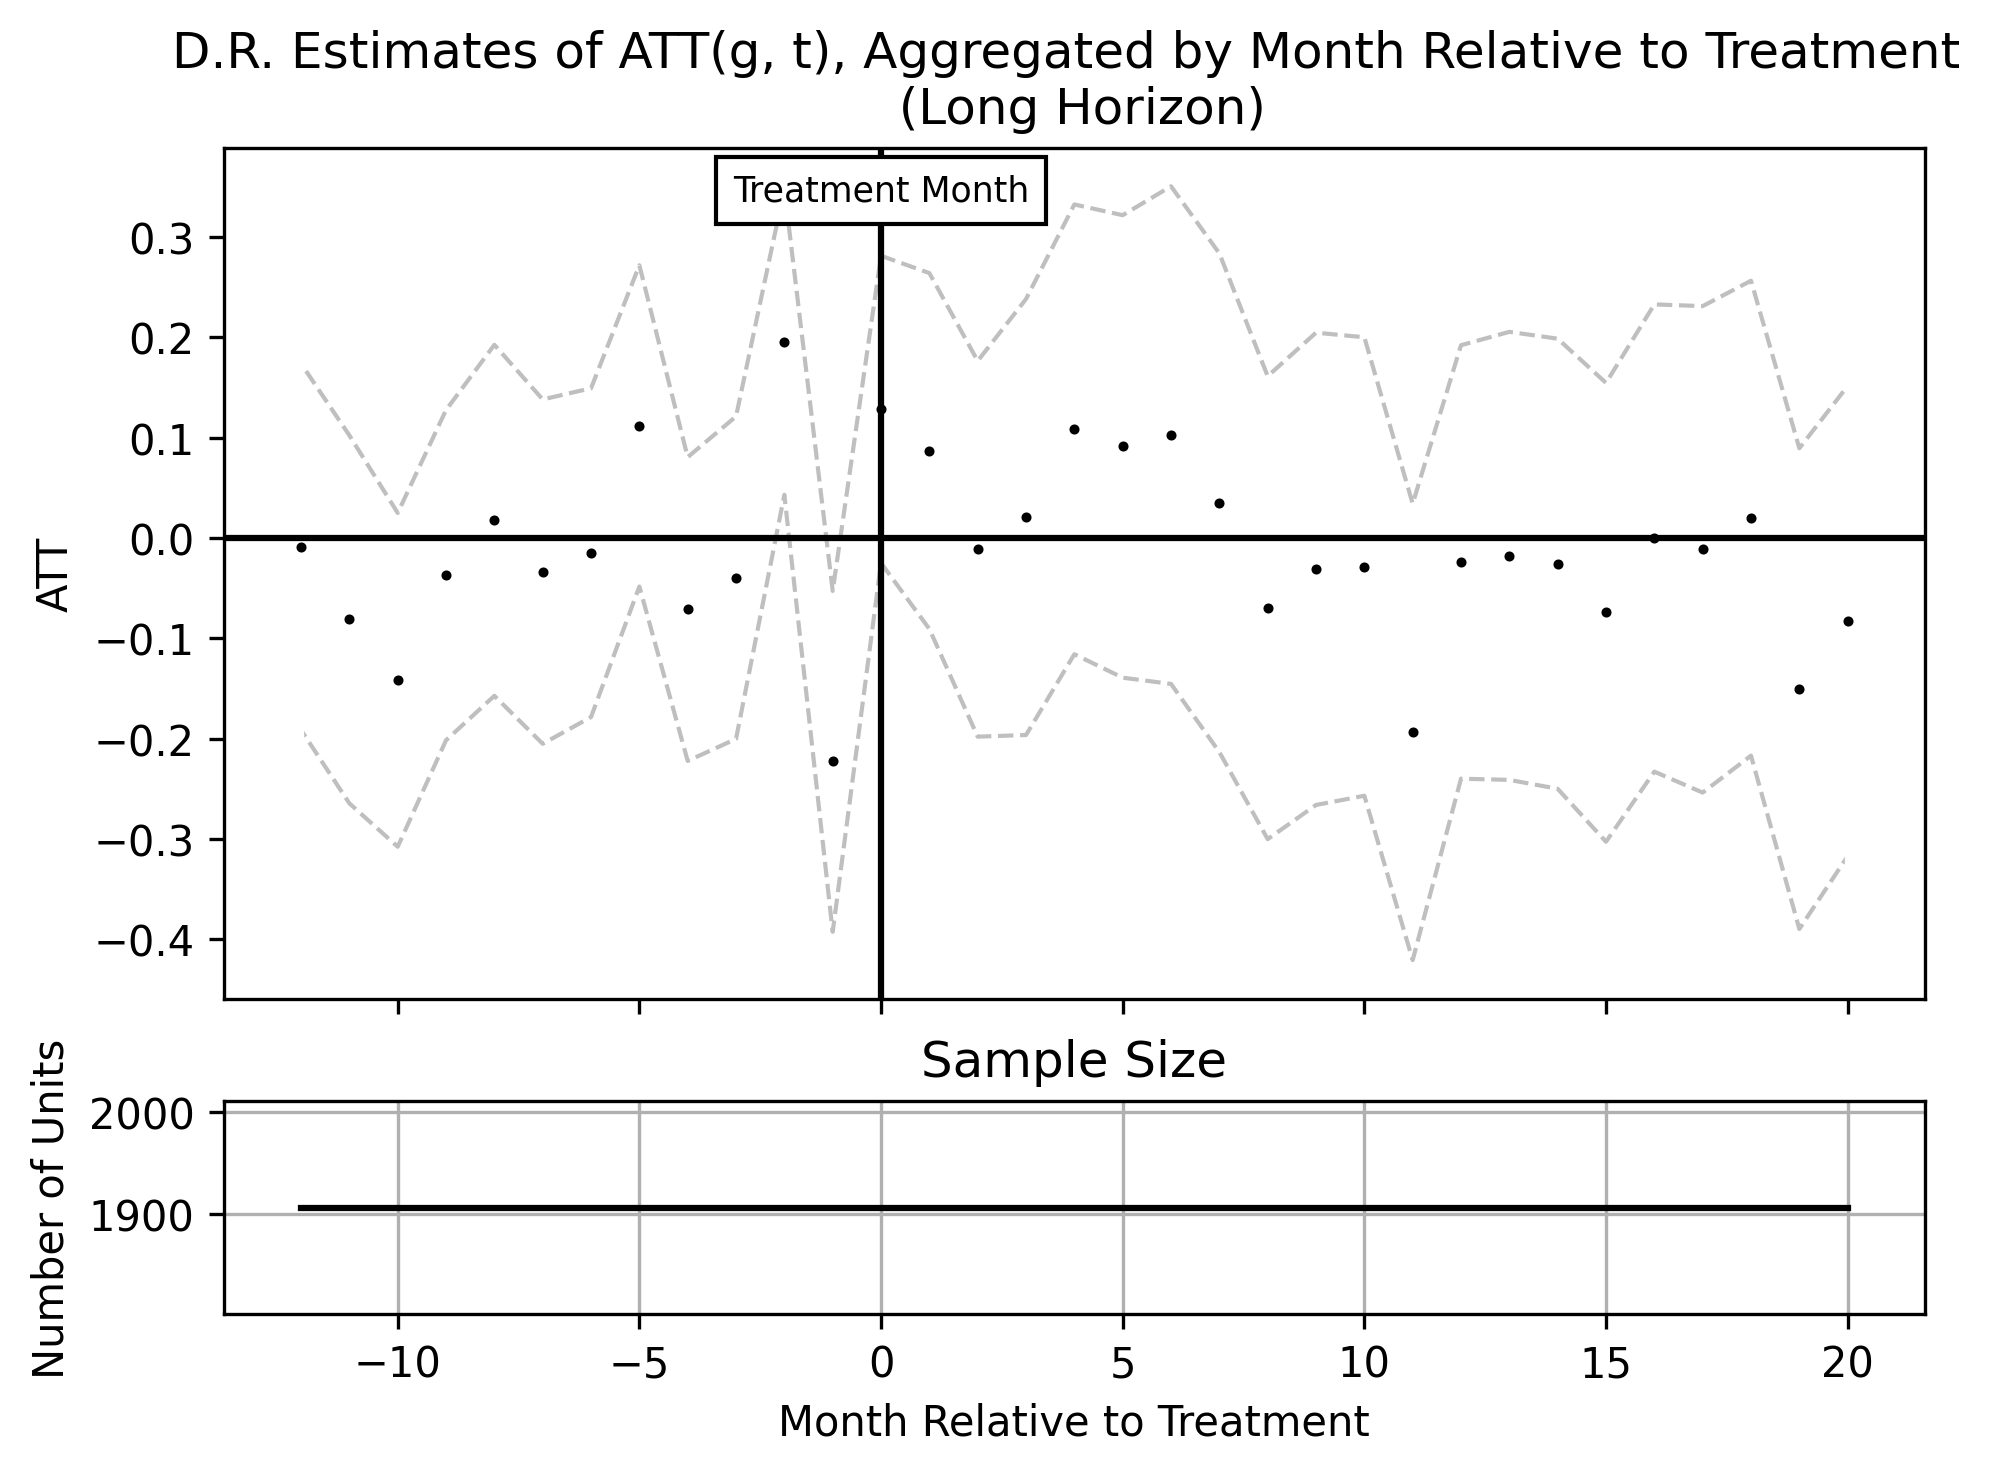
\includegraphics[scale=0.6]{output/all.png}
        \label{tab:my_label}
    \end{table}
\end{frame}
\begin{frame}{Results: Assaults}
    
    \begin{table}[H]
        \centering
        \tiny
        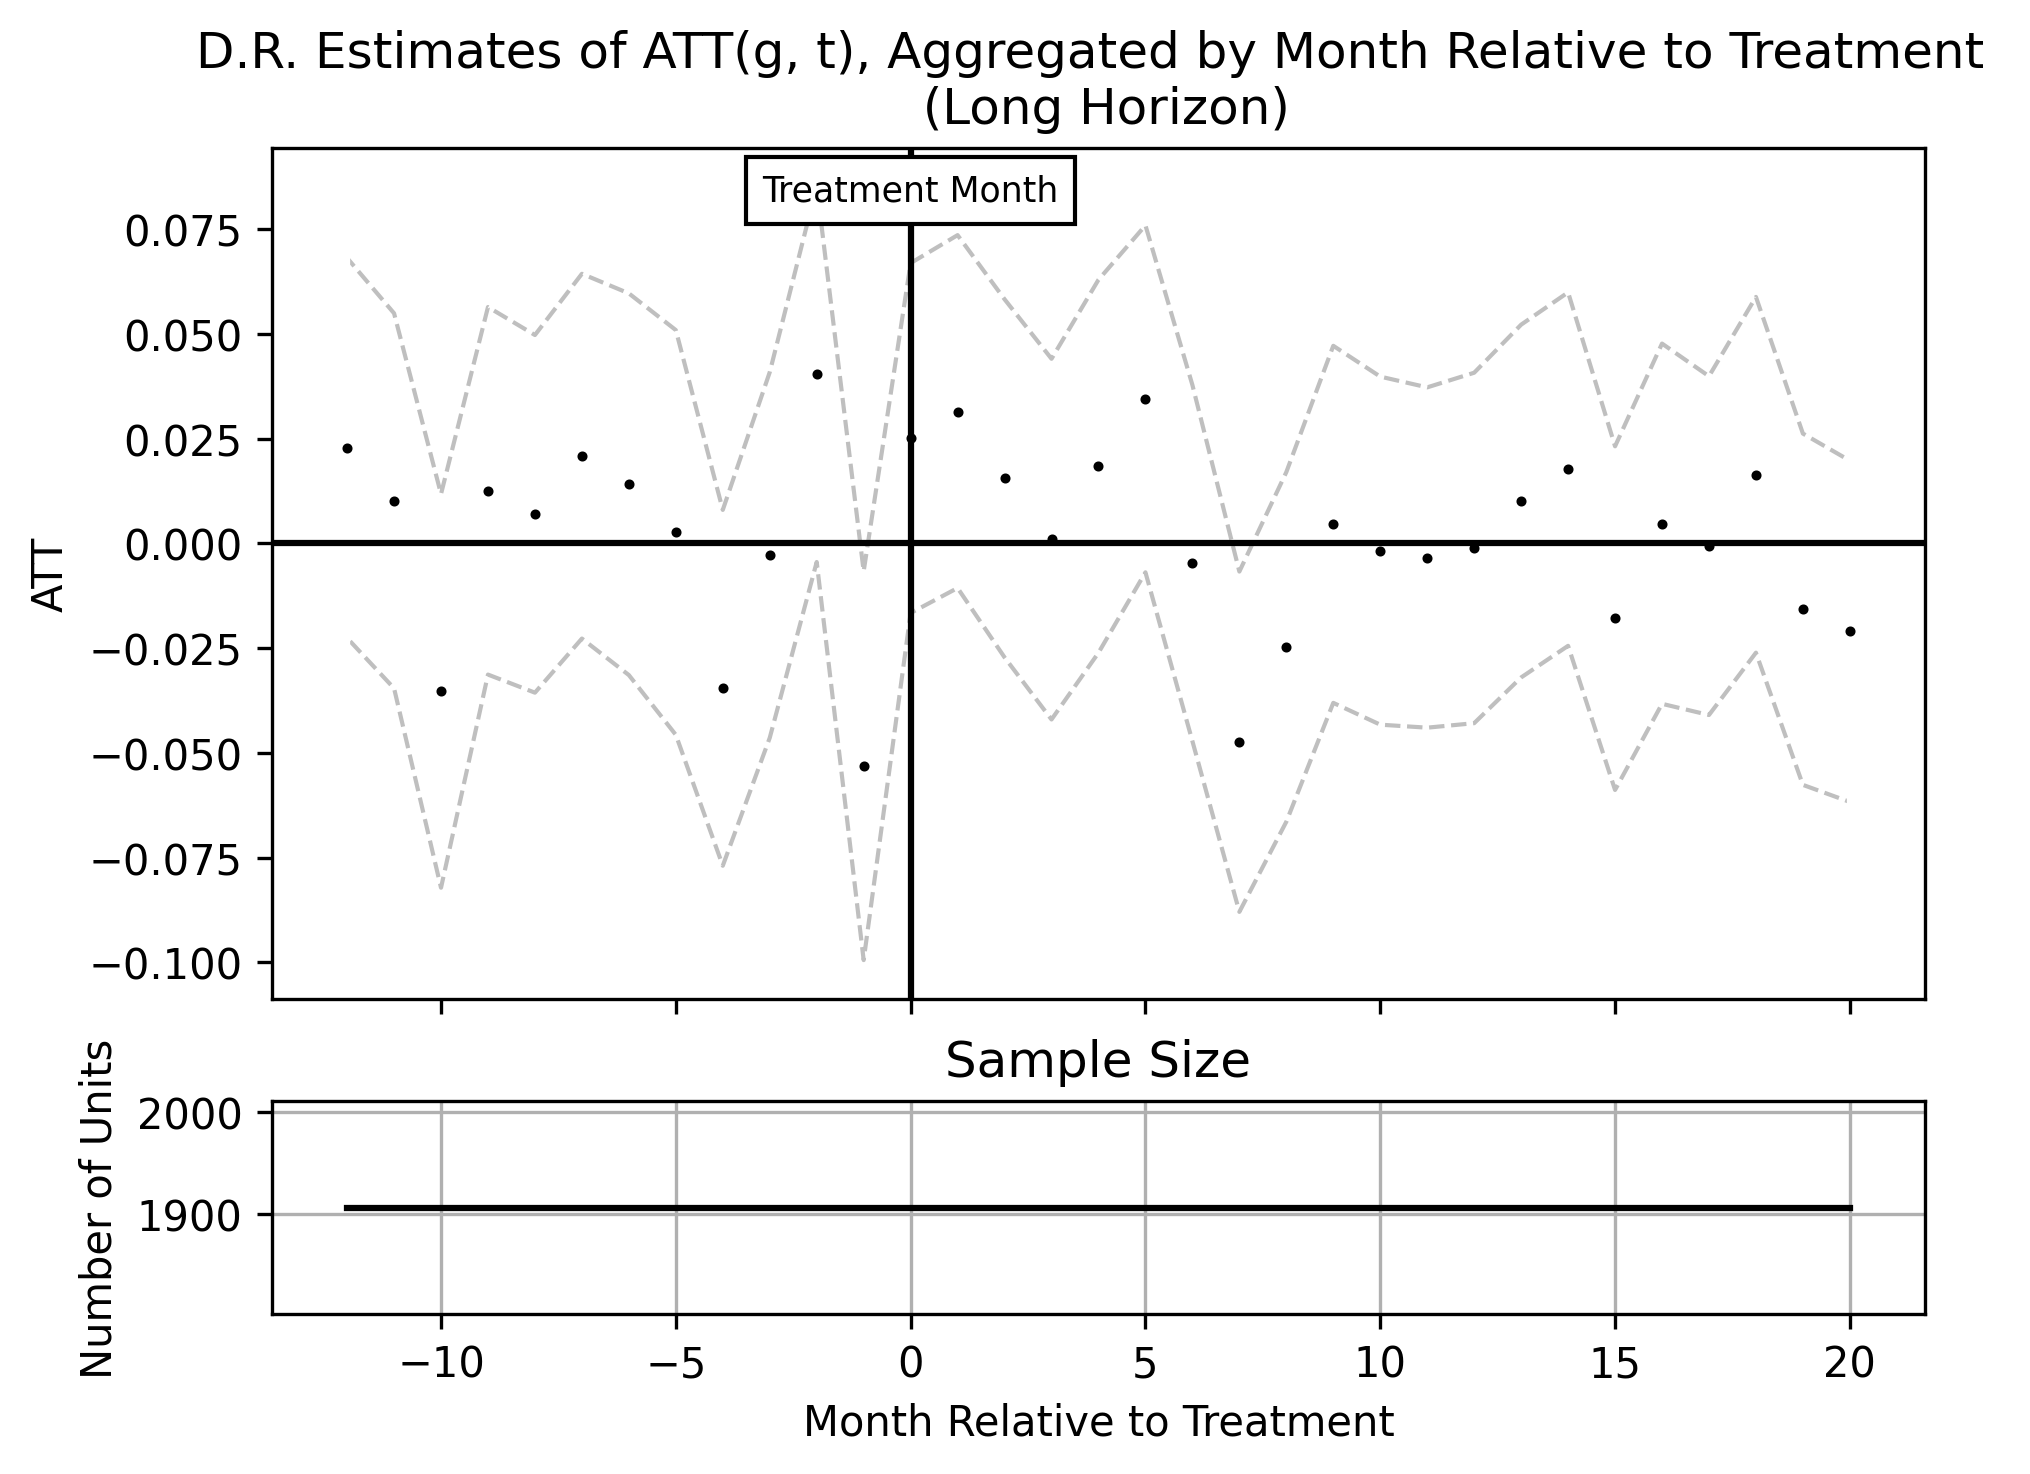
\includegraphics[scale=0.6]{output/assaults.png}
        \label{tab:my_label}
    \end{table}
\end{frame}
\begin{frame}{Results: Investigations}
    
    \begin{table}[H]
        \centering
        \tiny
        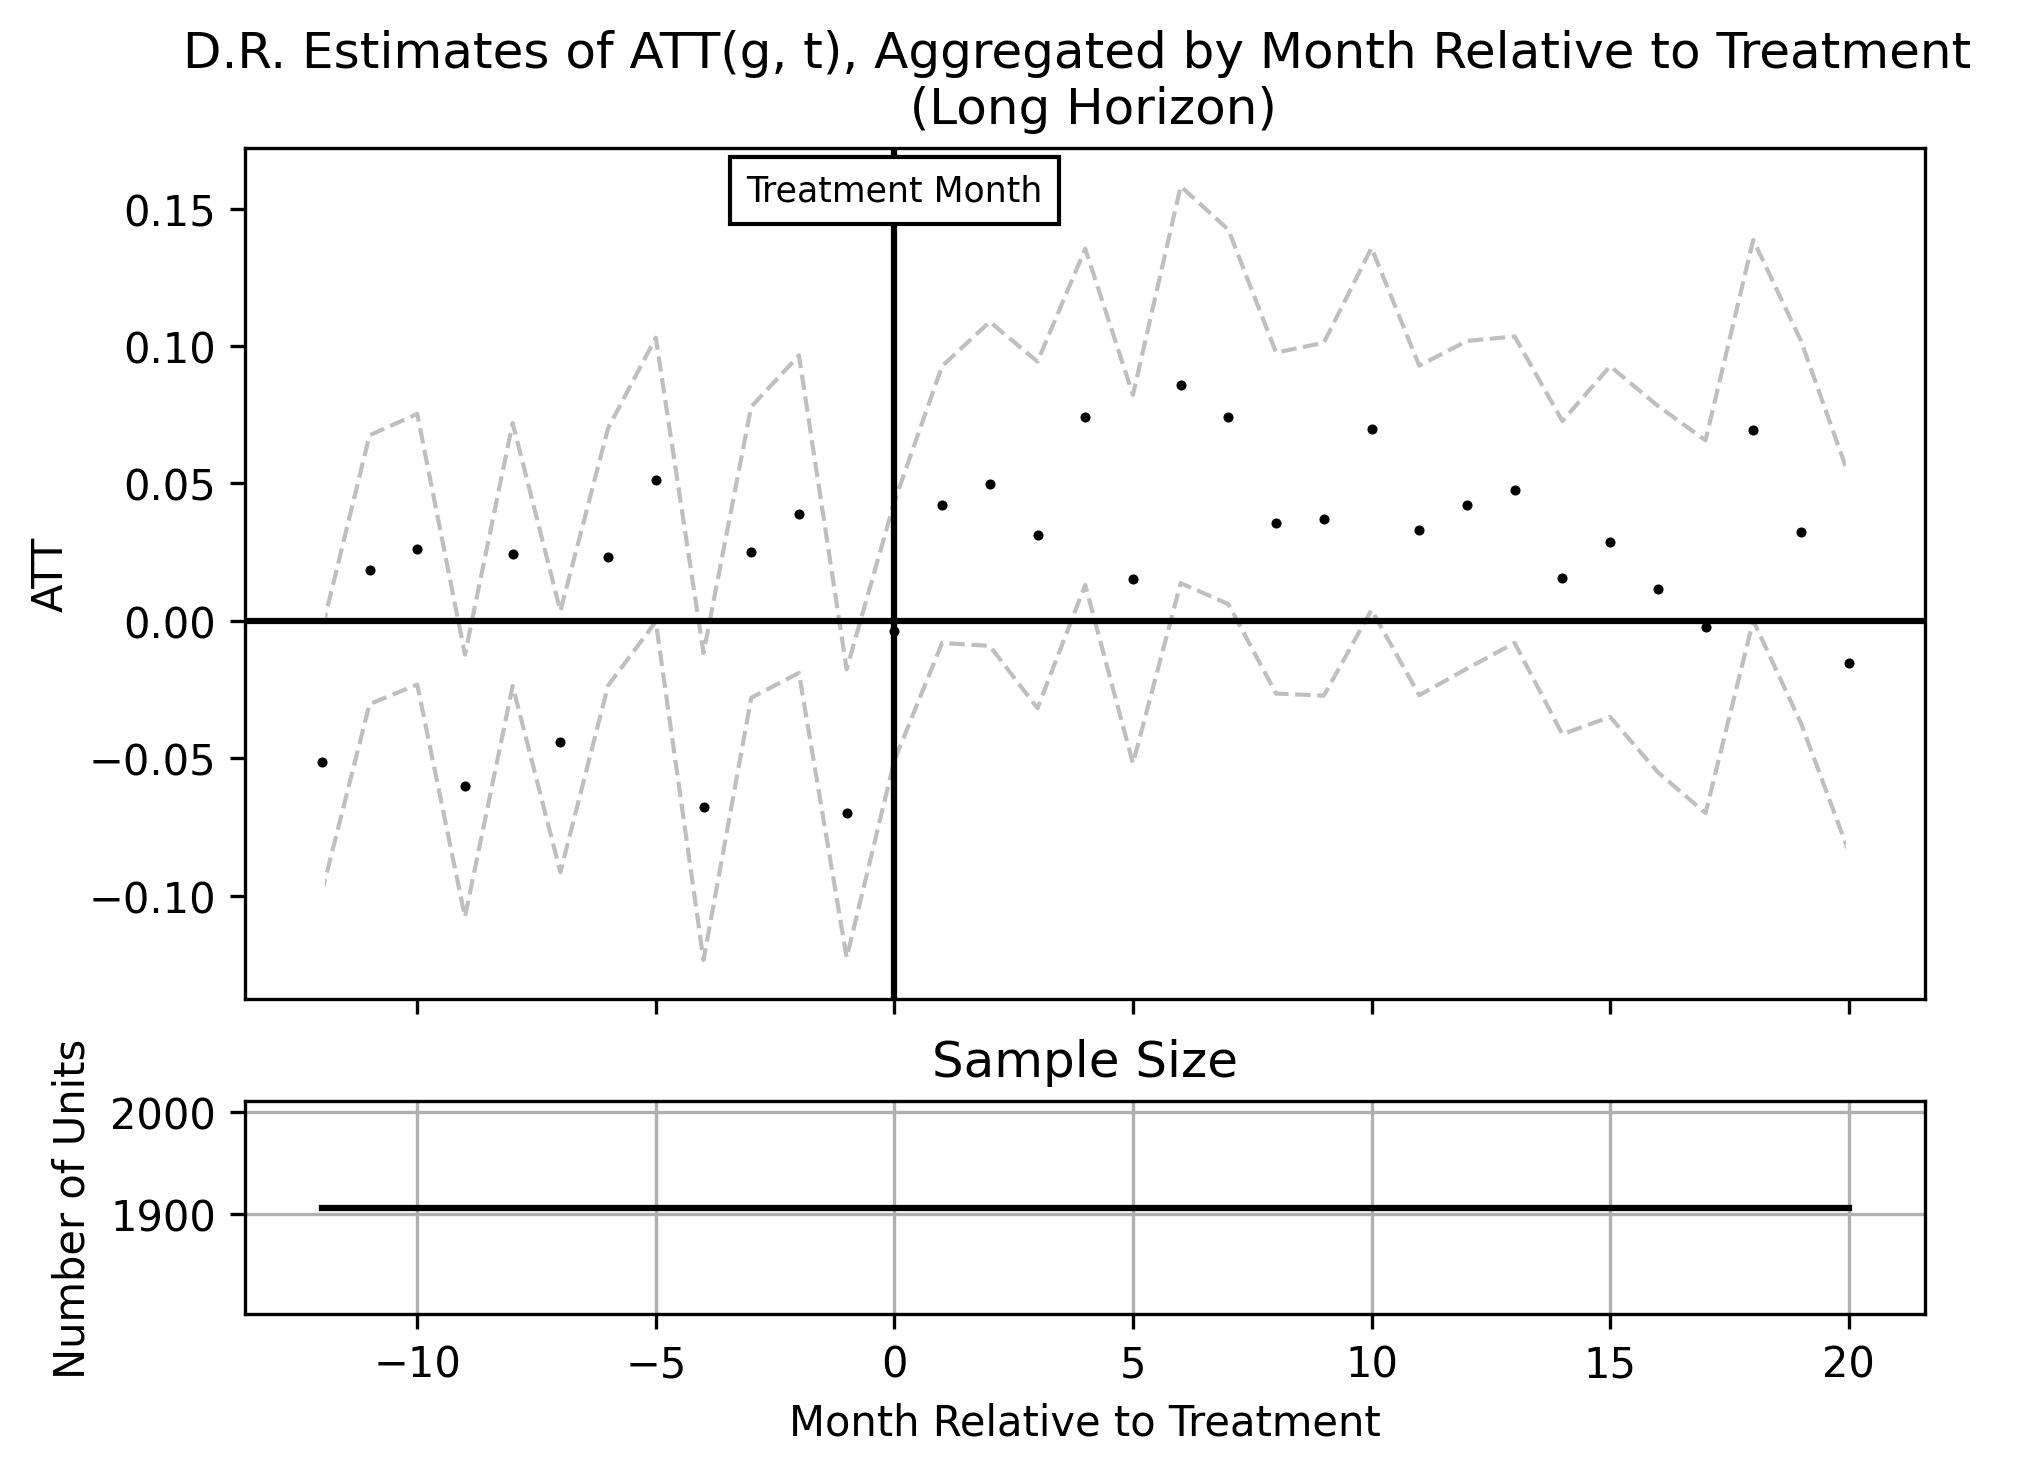
\includegraphics[scale=0.6]{output/investigations.png}
        \label{tab:my_label}
    \end{table}
\end{frame}



\begin{frame}{Next Steps}
    \begin{enumerate}
        \item Robustness checks

        \item Qualitiative analysis of what is happening in the 2 months before filing
        \item Am I double counting crimes?
    \end{enumerate}
\end{frame}

\end{document}
Close
